% Created 2024-08-05 lun 00:16
% Intended LaTeX compiler: pdflatex
\documentclass{article}
\usepackage[utf8]{inputenc}
\usepackage[T1]{fontenc}
\usepackage{graphicx}
\usepackage{grffile}
\usepackage{longtable}
\usepackage{wrapfig}
\usepackage{rotating}
\usepackage[normalem]{ulem}
\usepackage{amsmath}
\usepackage{textcomp}
\usepackage{amssymb}
\usepackage{capt-of}
\usepackage{hyperref}
\usepackage{fancyhdr}
\usepackage[top=25mm, left=25mm, right=25mm]{geometry}
\usepackage{longtable}
\fancyhead[R]{}
\setlength\headheight{43.0pt}
\usetheme{default}
\author{Luis Enrique Pérez S}
\date{2024-07-}
\title{Taller Almacenamiento Externo}
\hypersetup{
 pdfauthor={Luis Enrique Pérez S},
 pdftitle={Taller Almacenamiento Externo},
 pdfkeywords={},
 pdfsubject={},
 pdfcreator={Emacs 27.1 (Org mode 9.7.5)}, 
 pdflang={Español}}
\begin{document}

\maketitle
\fancyhead[C]{\includegraphics[scale=0.05]\\
ESCUELA POLITÉCNICA NACIONAL\\FACULTAD DE INGENIERÍA DE SISTEMAS\\
ARQUITECTURA DE COMPUTADORES}
\thispagestyle{fancy}


\section{Objetivos}
\label{sec:org906b069}

\begin{itemize}
\item Familiarizar al estudiante con herramientas de visualización de ocupación del disco duro
\end{itemize}

\section{Instrucciones}
\label{sec:org63d7c20}
\begin{enumerate}
\item Si dispone de un sistema operativo Windows instale el programa
\href{https://windirstat.net/download.html}{WinDirStat} o en su defecto, si dispone de un sistema operativo
Linux, puede ocupar la herramienta \emph{Disk} o instalar \href{https://installati.one/install-qdirstat-ubuntu-20-04/}{qdirstat}:
\end{enumerate}

\section{Captura}
\label{sec:orgc041e26}
\begin{center}
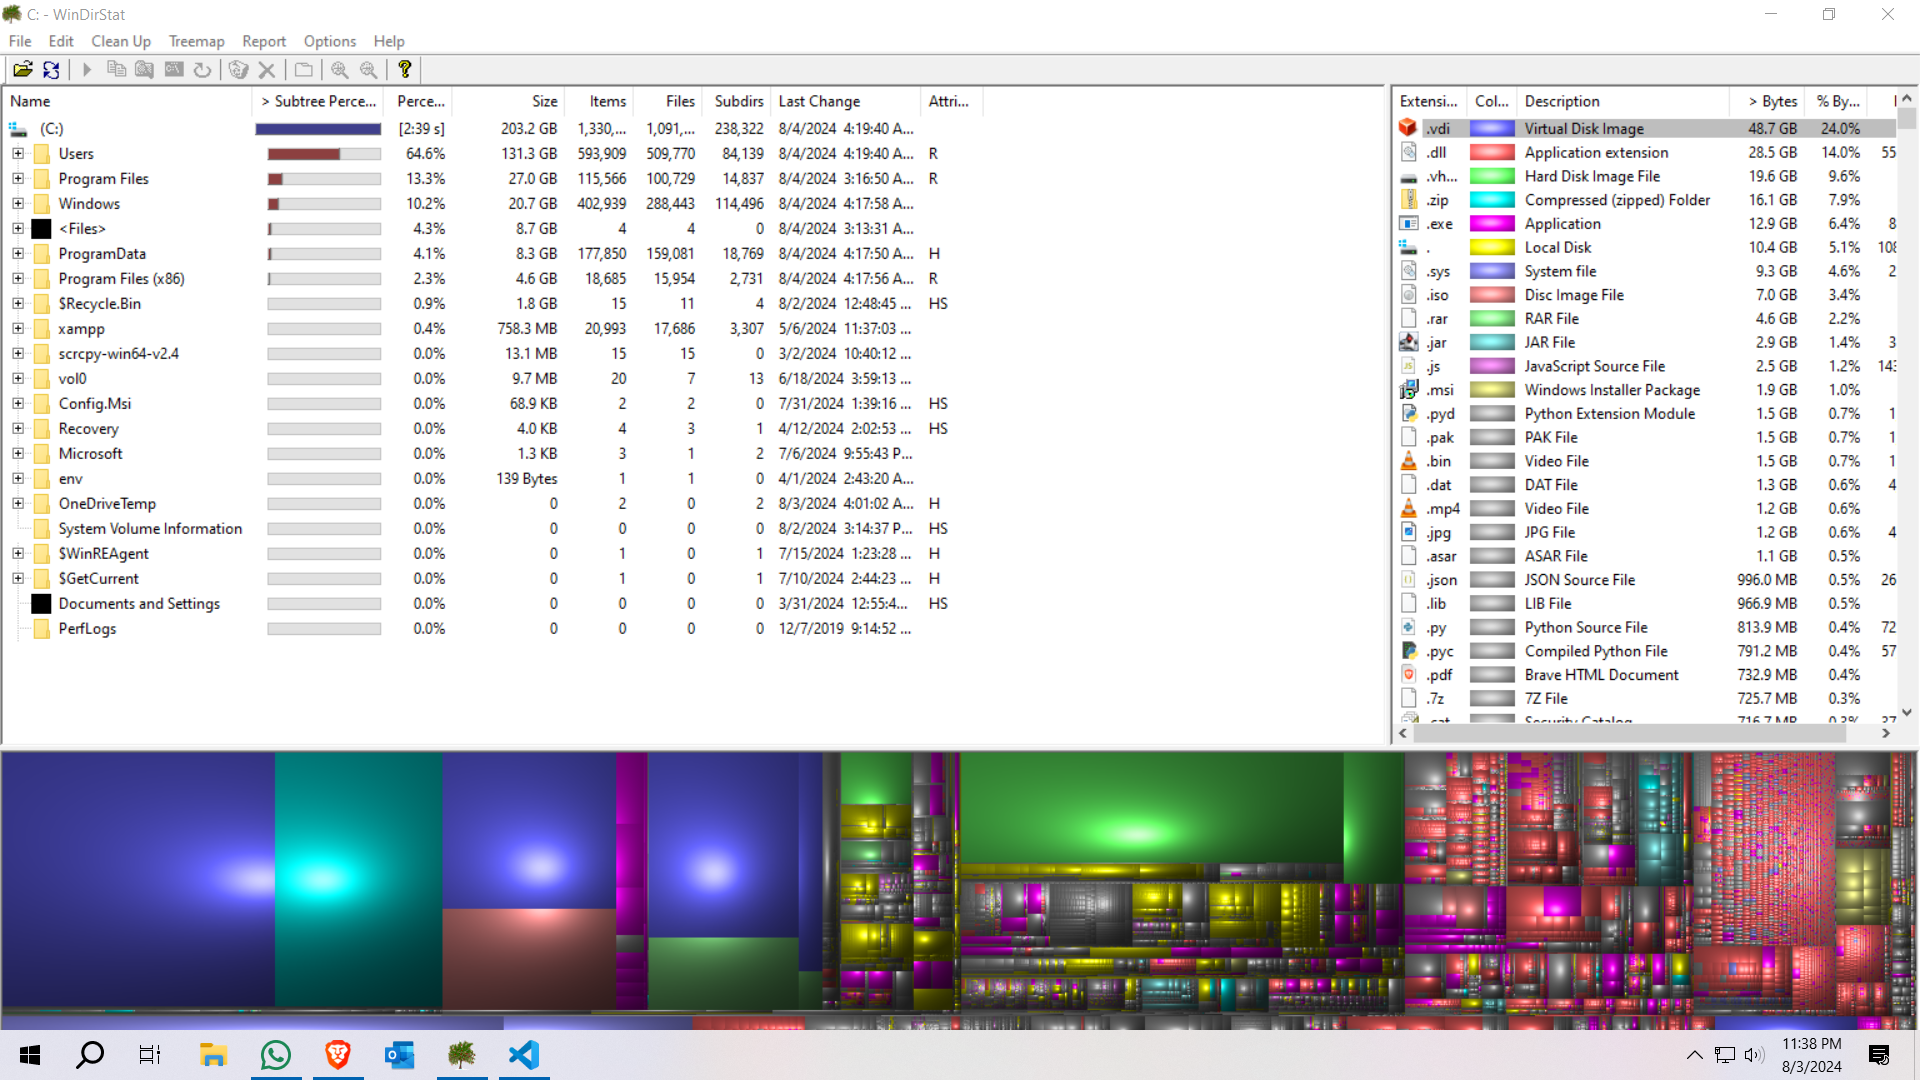
\includegraphics[width=.9\linewidth]{./WinDirStat.png}
\end{center}

\section{Preguntas 1}
\label{sec:orgcfa1f5f}
\begin{enumerate}
\item ¿En qué puede servirle programas como qdirstat o WinDirStat?
\end{enumerate}
Analizar el uso del disco de almacenamiento, como el uso del espacio (archivos pesados), administrar el almacenamiento, etc.
\begin{enumerate}
\item ¿Cómo opera el mapa que los programas proveen? Describa sus observaciones.
\end{enumerate}
Permite visualizar cada archivo y carpeta como un bloque o rectángulo en el mapa. Cada bloque está proporcionalmente dimensionado según el tamaño del archivo o carpeta que representa. Esto permite al usuario ver de un vistazo qué elementos están ocupando más espacio.

\section{Preguntas 2}
\label{sec:orgc90f806}
\begin{enumerate}
\item Luego de usar el programa ha podido establecer conclusiones sobre
su uso del espacio de disco duro, escriba tres conclusiones
relevantes

\item Archivos .dvi muy pesados
\item Mala organización de los archivos
\item Muchos archivos .zip guardados (16GB)
\end{enumerate}
\end{document}
